

\begin{center}\LARGE{\textsc{STAGE OLYMPIQUE DE MONTPELLIER 2016}}
\vrule depth 0pt height 0.4pt width 16cm\end{center}


%\medskip

\begin{center}
\includegraphics[scale=0.3]{logos/animath.jpg}
\end{center}

%\vspace*{0.5}

%\medskip

\begin{center}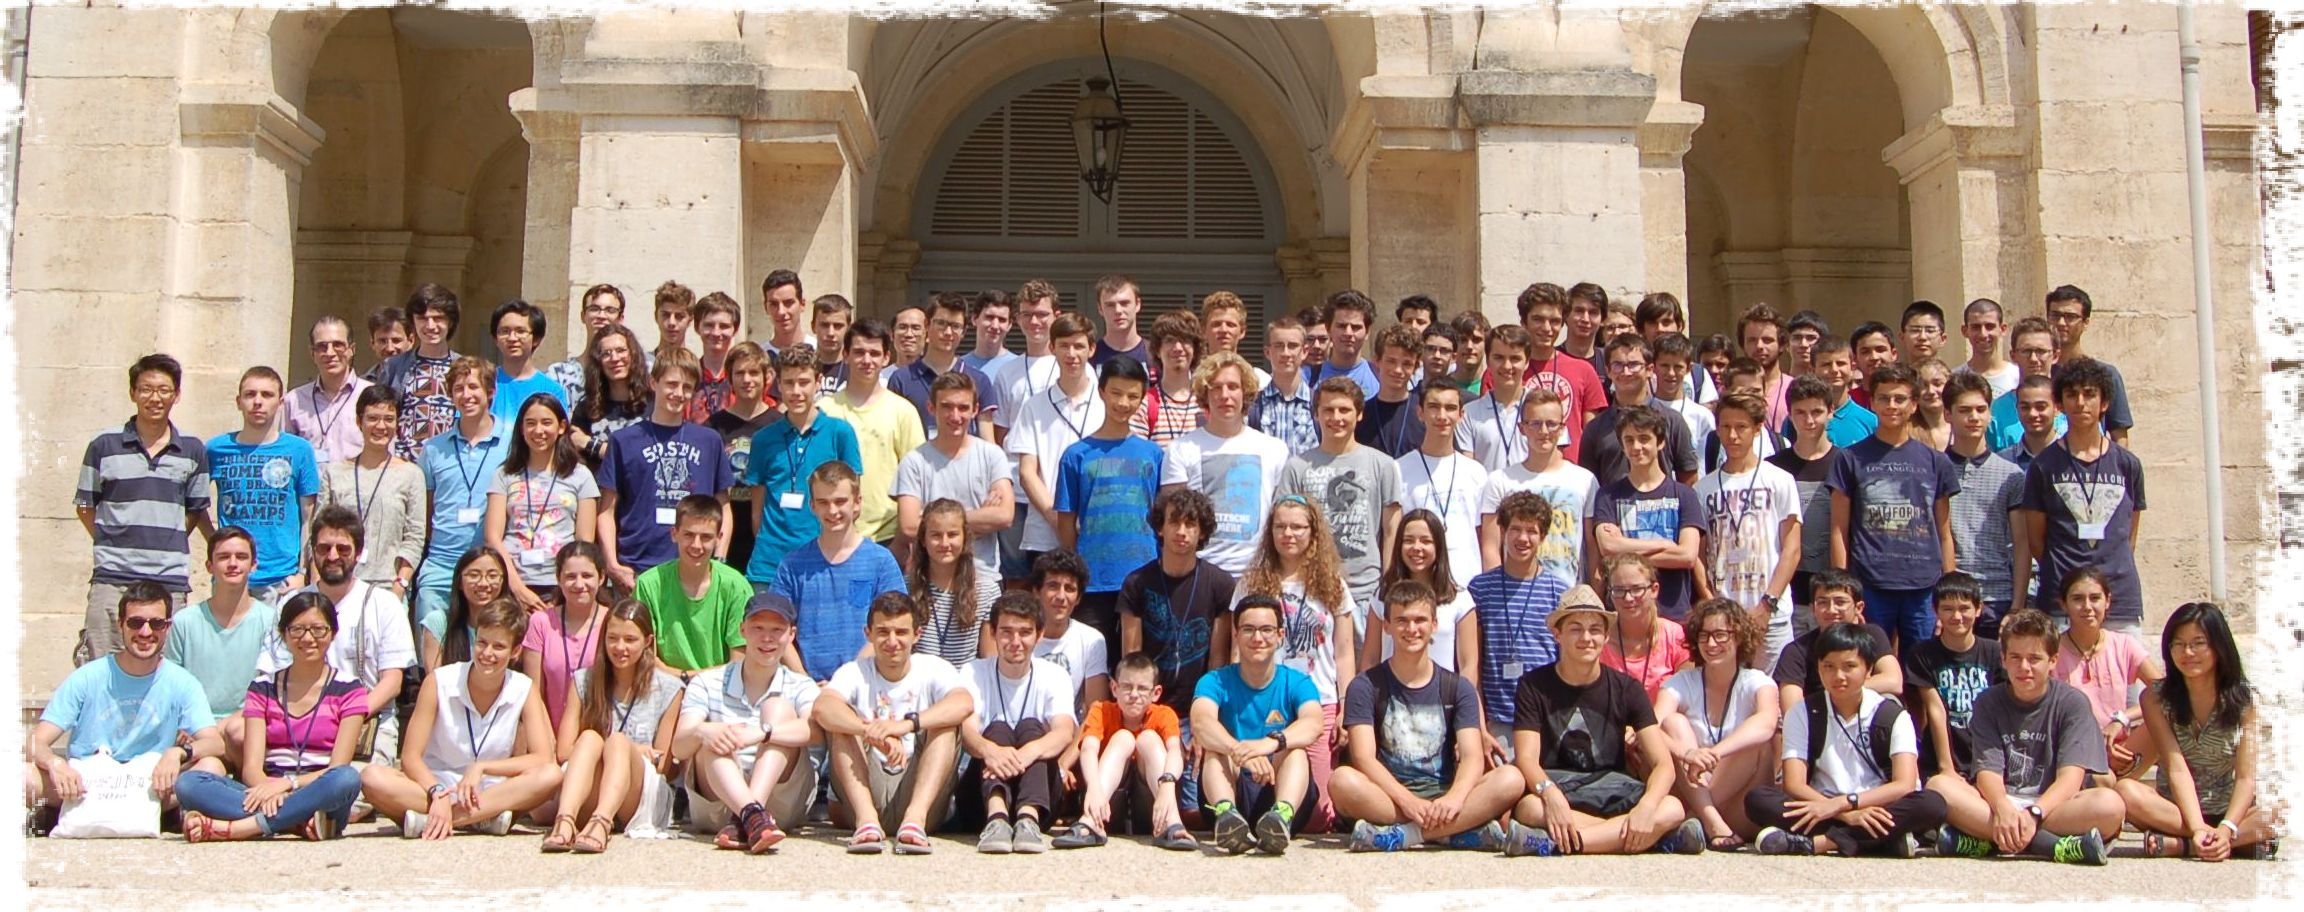
\includegraphics[width=16cm]{groupe.jpg}
\end{center}

%\vspace{0.5cm}

%\vspace*{0.5cm}
\begin{center}\large{du 16 au 26 août 2016}\end{center}




\begin{figure*}[h!]

   \begin{minipage}[c]{2cm}
   \centering
        
\includegraphics[width=2cm]{logos/EN.jpg}
   \end{minipage} \hfill
   \begin{minipage}[c]{2cm}
   \centering
      
\includegraphics[width=2cm]{logos/PAI.jpeg}
   \end{minipage} \hfill
   \begin{minipage}[c]{2cm}
   \centering
      
\includegraphics[width=2cm]{logos/CAPMATH_Logo_2Coul.pdf}
   \end{minipage} \hfill
      \begin{minipage}[c]{2cm}
   \centering
      
\includegraphics[width=2cm]{logos/inria.jpg}
   \end{minipage}
%   \hfill
%   \begin{minipage}[c]{2cm}
%   \centering
%      \includegraphics[width=2cm]{logos/axa.jpg}
%   \end{minipage} 
   \hfill\begin{minipage}[c]{2cm}
   \centering
        
\includegraphics[width=2cm]{logos/cm.jpg}
   \end{minipage}  \hfill
   \begin{minipage}[c]{2cm}
   \centering
      
\includegraphics[width=2cm]{logos/casio.jpg}
   \end{minipage}

\end{figure*}



\pagebreak

\pagestyle{empty}~

 \pagebreak



\clearpage

\vspace*{\stretch{1}}

\begin{flushright}

\textbf{\Large{Avant-propos}}

\bigskip

\emph{Le stage olympique de Montpellier 2016 a été organisé par l'association Animath.}

\bigskip

\emph{Son objet a été de rassembler 83 collégien-ne-s et lycéen-ne-s de quatrième à première, \\ de ??? à ??? ans, passioné-e-s de mathématiques \\ sélectionnés parmi les quelque ??? candidats à la COUPE ANIMATH, \\ dont certains  représenteront la France aux compétitions internationales : \\
Olympiades Internationales de Mathématiques (IMO), \\ Olympiades Balkaniques Junior de Mathématiques (JBMO), \\ Olympiades Européennes de Filles de Mathématiques (EGMO), \\ Romanian Masters of Mathematics (RMM), \\ Olympiades Mathématiques du Bénélux (BxMO), \\ Mediterranean Youth Mathematical Championship (MYMC). \\ Un certain nombre d'autres animateurs et stagiaires \\ ont déjà participé à l'une des compétitions ci-dessus.}
 
\bigskip

\emph{Tous les animateurs sont bénévoles.} 
\end{flushright}

\vspace*{\stretch{1}}



\pagebreak

\mbox { }

\pagebreak
